\documentclass[11pt,english,a4paper]{article}
\usepackage[right=3.6cm,left=3.6cm,bottom=3.6cm,top=3.6cm]{geometry}
\usepackage{mathpazo}
\renewcommand{\sfdefault}{lmss}
\renewcommand{\ttdefault}{lmtt}
\renewcommand{\familydefault}{\rmdefault}
\usepackage[T1]{fontenc}
%\usepackage[utf8]{inputenc}
\usepackage[utf8x]{inputenc}
\usepackage{lmodern,textcomp}
\setlength{\parskip}{\smallskipamount}
\setlength{\parindent}{0pt}
\usepackage{color}
\usepackage[english]{babel}
\usepackage{graphicx}
\usepackage{amsmath}
\usepackage{amsthm}
\usepackage{array}
\usepackage[unicode=true,bookmarks=true,bookmarksnumbered=true,
 bookmarksopen=true,bookmarksopenlevel=4,breaklinks=true,pdfborder={0 0 0},
 backref=false,colorlinks=false]{hyperref}
\hypersetup{pdftitle={SINF2345 Languages and Algorithms for Distributed Applications - Project report},pdfauthor={Martin Trigaux -- Bernard Paulus}}
\usepackage{breakurl}
\usepackage{todonotes}

\sloppy

%% DOCUMENT %%
\begin{document}
\title{SINF2345 Languages and Algorithms for Distributed Applications \\ Project report}
\author{
  \begin{tabular}{c c}
    Martin \textsc{Trigaux}  &  Bernard \textsc{Paulus} \\
    \small SINF22MS                 &  \small SINF22MS \\
    \small \href{mailto:martin.trigaux@student.uclouvain.be}{martin.trigaux@student.uclouvain.be}  &  
    \small \href{mailto:bernard.paulus@student.uclouvain.be}{bernard.paulus@student.uclouvain.be}
  \end{tabular}
}
\date{\emph{\today}}
\maketitle

\tableofcontents  
\section*{Introduction}
The aim of the project is to build a distributed banking system. % QUESTION : Usefull to remind the full mission ?
The system is distributed in a way such that any bank node is award of the full banking system state at all time but only atomics messages are transfered between nodes.\\

To build this project, we decided to use the programming language Erlang.
We believe this language is highly adequate for concurrent applications and that is what motivated us to use it for this project.
This language handles also very well events and made easier the implementation of proposed algorithms in the reference book.

\section{Architecture}
\begin{figure}[h]\centering
  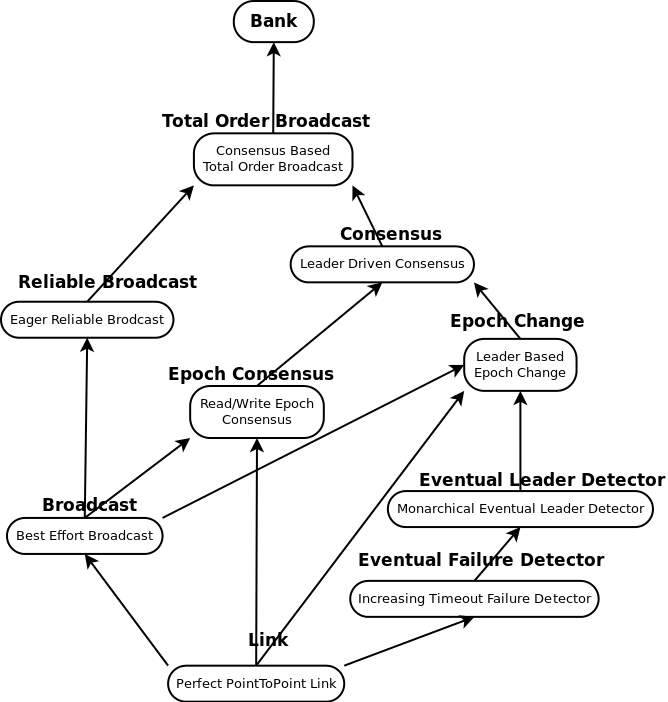
\includegraphics[width=\textwidth]{arch.png}
\end{figure}
To realise the distributed system, we used the reference book ``Reliable and Secure Distributed Programming'' by C. Cachin, R. Guerraoui and L. Rodrigues second edition.
As the modules and algorithms are tested and well defined, we tried to stick as much as possible to the book and implemented several algorithms from it.
We used a architecture based on layers and encapsulation of messages.
Each module is connected to other and behave upon events (recieved messages from other modules).

\subsection*{Basic abstractions}
We used the \textbf{perfect link} module\footnote{Module 2.3 p37 in reference book} for basic point to point communications.
These are at the lowest level of our architecture and simply transmit messages to above modules.
The perfect link ensures \emph{reliability} and the \emph{no duplication} property.\\

To handle failing nodes in a partially synchronous system, we used an \textbf{eventual failure detector} module\footnote{Module 2.8 p54 in reference book}.
This was implemented using the \textbf{increasing timeout failure detector} algorithm\footnote{Algorithm 2.7 p55 in reference book}.\\

Once we have successfully detected faulty processes, we can focus on correct ones and elect a leader.
The \textbf{eventual leader detector} module\footnote{Module 2.9 p56 in reference book} allows to elect a reliable as a leader to perform certain computations on behalf of the others.
We implemented the \textbf{monarchical eventual leader detector} algorithm\footnote{Algorithm 2.8 p58 in reference book}.
This algorithm elect the leader with the highest rank among the alived nodes with the possibility to restore suspected nodes (eg: too slow to reply and were wrongly suspected as failing).

\subsection*{Broadcasts}
We used the \textbf{best effort broadcast} module\footnote{Module 3.1 p75 in reference book} for implement the broadcast messages between nodes.
This module transmit messages to the adequate perfect links.
As we want to handle failing nodes, we used a \textbf{reliable broadcast} algorithm\footnote{Module 3.2 p77 in reference book}.
To ensure the \emph{agreeement} property, we implemented the \textbf{eager reliable broadcast} algorithm\footnote{Algorithm 3.3 p80 in reference book}.


\subsection*{Consensus}
As we are working in a concurrent system, we need to reach to a \textbf{consensus} and decide the next state of the system.
We used the \textbf{epoch-change} abstraction\footnote{Module 5.3 p218 in reference book} to take a decision on a proposed value.
This was implemented using the \textbf{leader based epoch change} algorithm\footnote{Algorithm 5.5 p219 in reference book}.
We encounters majors problem using this algorithm due to an error in the reference book.
This was disccused in an furthur errata of the book\footnote{See http://distributedprogramming.net/docs/Errata.pdf} we discovered only recently.
However the authors made the unexplicit assumption that the local stack of messages is FIFO.
That assumption was at first not verified and we realised later it is crucial for the success of the algorithm.
The implemented algorithm has been fixed using both the errata and the FIFO queuing process.\\

In the attempt to obtain a consensus, we used the \textbf{epoch consensus} module\footnote{Module 5.4 p221 in reference book}.
We implemented it using the \textbf{read write epoch consensus} algorithm\footnote{Algorithm 5.6 p223 in reference book}.
The algorithm uses timestamp in a state value so as to serves the \emph{validity} and \emph{lock-in} or the epoch consensus.
The method used relies on a majority if correct processes and assumes we have at least more than the half on non-failing nodes.
In the \textbf{leader driven consensus} algorithm\footnote{Algorithm 5.7 p225 in reference book}, we distinguish the instances of epoch consensus by their timestamp.
Once we receive a new epoch event and need to switch the epoch, the algorithm aborts the running epoch consensus and initialize the next epoch consensu using the state of the previous one.

\subsection*{Total order broadcast}
For our banking application, ne need to rely on a delivery order in case of concurrent transactions.
In the previous broadcast abstraction, we used FIFO-order broadcast but we had no assumption on the delivery order.
The \textbf{total order broadcast} module\footnote{Module 6.1 p283 in reference book} aims to fix this problem and order all messages, even those not from different senders.
This module was implemented using the \textbf{consensus based total order broadcast} algorithm\footnote{Algorithm 6.1 p285 in reference book}.
The system is based on consensus abstraction to be able, at any time, to decide on a set of unordered messages between two processes.

\subsection*{Banking system}
Once we have implemented all our modules, we can build our banking module on top of a reliable system.
Each bank node can handle users commands (account creation and money transfer).
Based on the rules specified (negative account fee), the bank node broadcast the adequate atomic messages to the banking network.
The transactions are validated only once the initial node recieves and acknowledgment of the other nodes.

\section{Manual}
To launch the program you will need the \texttt{erlang} package installed on your computer.
This as only been tested on Linux environments.
Open a terminal an go to the folder containing the code.
Compile the code using the command \texttt{make}.\\

To launch the code, use the following command :
\begin{verbatim}
$ erl -s test main
Erlang R15B01 (erts-5.9.1) [source] [64-bit] [smp:2:2] [async-threa\
ds:0] [hipe] [kernel-poll:false]

Eshell V5.9.1  (abort with ^G)
1>

Banking application with 3 nodes

Creating nodes 1 and 2
Transfering money from #1 to #2
2>
\end{verbatim}
At this state, three banks node are running.
The accounts 1 and 2 have been created with respectively 10 and 20 units of money (let's say € for the sake of simplicity).
5€ have then been transfered from the account 1 to 2.\\

For deeper testing, the users can interact with the bank nodes using the erlang shell interface.
Launch the shell prompt using simply the \texttt{erl} command and load the module using \texttt{test:main().} or \texttt{test:main(INT).} for a custom number of nodes.
The result of the function needs is a list that needs to be stored in a list.
\begin{verbatim}
1> [A, B, C] = test:main(3).
\end{verbatim}

To create a new account use the command \texttt{bank:create\_account(\#BANK, \#ID, \#MONEY).}.
For example \texttt{bank:create\_account(B, 3, 5).} to create a third account with 5€ on it using the second bank (don't forget the ending dot).\\

To transfer money from an account to another, use the command  \texttt{bank:transfer\_money(\#BANK, \#IDFROM, \#IDTO, \#MONEY).}.
For example \texttt{bank:transfer\_money(C, 2, 3, 5).} to transfer 5€ from the second account to the third one using the third bank node.\\

To display the amount on the account of the user, use the command  \texttt{bank:check\_account(\#BANK, \#ID).}.
For example \texttt{bank:check\_account(A, 1).} to check the amount on the account of the first user using the first bank.\\

\begin{verbatim}
$ erl
...
1> [A, B, C, D] = test:main(4). %% 4 bank nodes, 2 accounts, 1 transfer
2> bank:create_account(C,3,10). %% create 3rd account
3> bank:transfer_money(D,3,1,5). %% transfer 5€ 3 -> 1
4> bank:check_account(B,3).
Account 3 has 5€ leftok
\end{verbatim}

\section{Conclusion}
The choice of Erlang as the choosen programming language allowed us to build a fully concurrent system.
On the other hand, we couldn't use the proposed framework and had to reimplement several algorithms in the book.
This project was quite interresting as it made us work with several different abstractions and different layers of our application.
After this project, we believe we obtained a robust stack that could be reused to different applications.

\end{document}
